Statistical errors are obtained via Gaussian error propagation. 

The error of an extrapolation of a linear fit is obtained by first shifting the data to the "center-of-mass" frame given by $(x,y) \to (x,y) - (\bar{x},\bar{y})$, with $(\bar{x},\bar{y}) = \frac{\sum_i \frac{(x_i,y_i)}{(\Delta y_i)^2}}{\sum_i \frac{1}{(\Delta y_i)^2}}$\footnote{Here we assume that $x_i$ has no error. This will be the case for all fits.}, because in this frame the covariance between the slope an the offset vanishes.

\subsection{Part 1}
\subsubsection{Assignment 3 - myon energy loss}

\begin{table}
\centering
\caption{Myon momentum in inner and outer detector}
\begin{tabular}{ccc}
\toprule
n & $p_{in}/\si{GeV}$ & $p_{out}/\si{GeV}$\\
\midrule
1 & / & /\\
2&	-85&	-53.92\\
3&	43.4&	43.83\\
4&	-241.37&	-237.02\\
5&	48.89&	44.77\\
6&	-168.16&	-177.62\\
7&	117.32&	96.56\\
8&	-71.94&	-64.96\\
9&	199.91&	199.44\\
10&	-57.84&	-50.01\\
11&	/ & /\\
12&-100.75&	-94.11\\
13&	38.26&	34.48\\
14&	-105.19&	-108.68\\
15&	236.12&	236.61\\
16&	-131.69&	-125.51\\
17&	152.24&	157.69\\
18&	-35.23&	-32.18\\
19&	54.19&	50\\
20&	-84.75&	-68.09\\
21&	104.26&	107.98\\
22&	-184.01&	-170.66\\
23&	100.36&	101.13\\
\bottomrule
\end{tabular}
\label{tab:task1_myon}
\end{table}

In tabular \ref{tab:task1_myon} the measured momentum in the inner and outer detector part are given for the first 23 events. In event 1 and 11 the myon trace did not continue to the outer part. The energy loss is now given by $\Delta E = |p_{out}| - |p_{in}|$ (note that the myons can be treated like relativistic particles). The mean energy loss is given by $\Delta E = \si{(5 \pm 9)\,GeV}$.

\subsubsection{Assignment 6 - $Z_0 \to e^+ e^-$ invariant mass}
\begin{table}
\centering
\caption{Electron/positron momentum and the invariant mass $m$}
\begin{tabular}{ccccc}
\toprule
n & $p_1$/GeV & $p_2$/GeV & $m_1$/GeV & $m_2$/GeV\\
\midrule
1 &	-115.81&	63.29 & 171.23 & 171.23\\ 
2&	-49.69&	60.92 & 110.04 & 110.04\\
3&	-78.58&	101.01& 178.18 & 178.18\\
\bottomrule
\end{tabular}
\label{tab:task1_zee}
\end{table}

In tabular \ref{tab:task1_zee} the momentum of the $e^+/e^-$ is given together with the corresponding invariant mass. The invariant mass was calculated in two ways, first using the electron mass and second neglecting the electron mass. As one can see the electron mass does not have an influence on the invariant mass (So the electrons can be treated as ultra relativistic). 

\subsection{Part 2}
\begin{figure}
\centering
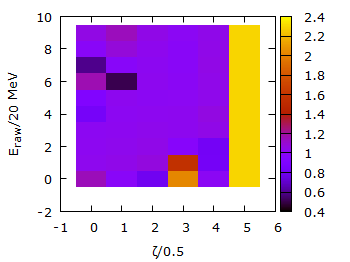
\includegraphics[scale=1]{data/zee_init/zee_init.png}
\caption{Correction factor $E_e/E_{\mathrm{raw}}$ over $E_{\mathrm{raw}}$ and $\eta$}
\label{fig:part2_factor}
\end{figure}

In figure \ref{fig:part2_factor} the correction factor $E_e/E_{\mathrm{raw}}$ is plotted over the raw energy $E_{\mathrm{raw}}$ and $\eta$. 

\subsection{Part 3 - W Boson mass}

\subsubsection{W boson mass}

The QCD scale factor was set to $\alpha = 0.33 \pm 0.01$ and the fit range $30 - 50 \si{GeV}$. We estimate the error on the fit range as $5 \si{Gev}$

In tabular \ref{tab:task3_33} the measured half maxima $h$ are given for several hypothetical masses of the W boson. This data will be used as a gauge curve for the mass.

\begin{table}
\centering
\caption{Measured half maxima $h$ for different W boson masses}
\begin{tabular}{ccccc}
\toprule
$m_W$/GeV & $h$/GeV & $\Delta h$/GeV\\ 
\midrule
75&	40.18&	0.06\\
78&	41.78&	0.07\\
79&	42.25&	0.06\\
80&	42.85&	0.06\\
81&	43.46&	0.07\\
82&	43.79&	0.07\\
85&	45.49&	0.11\\
\bottomrule
\end{tabular}
\label{tab:task3_33}
\end{table}

\begin{figure}
\centering
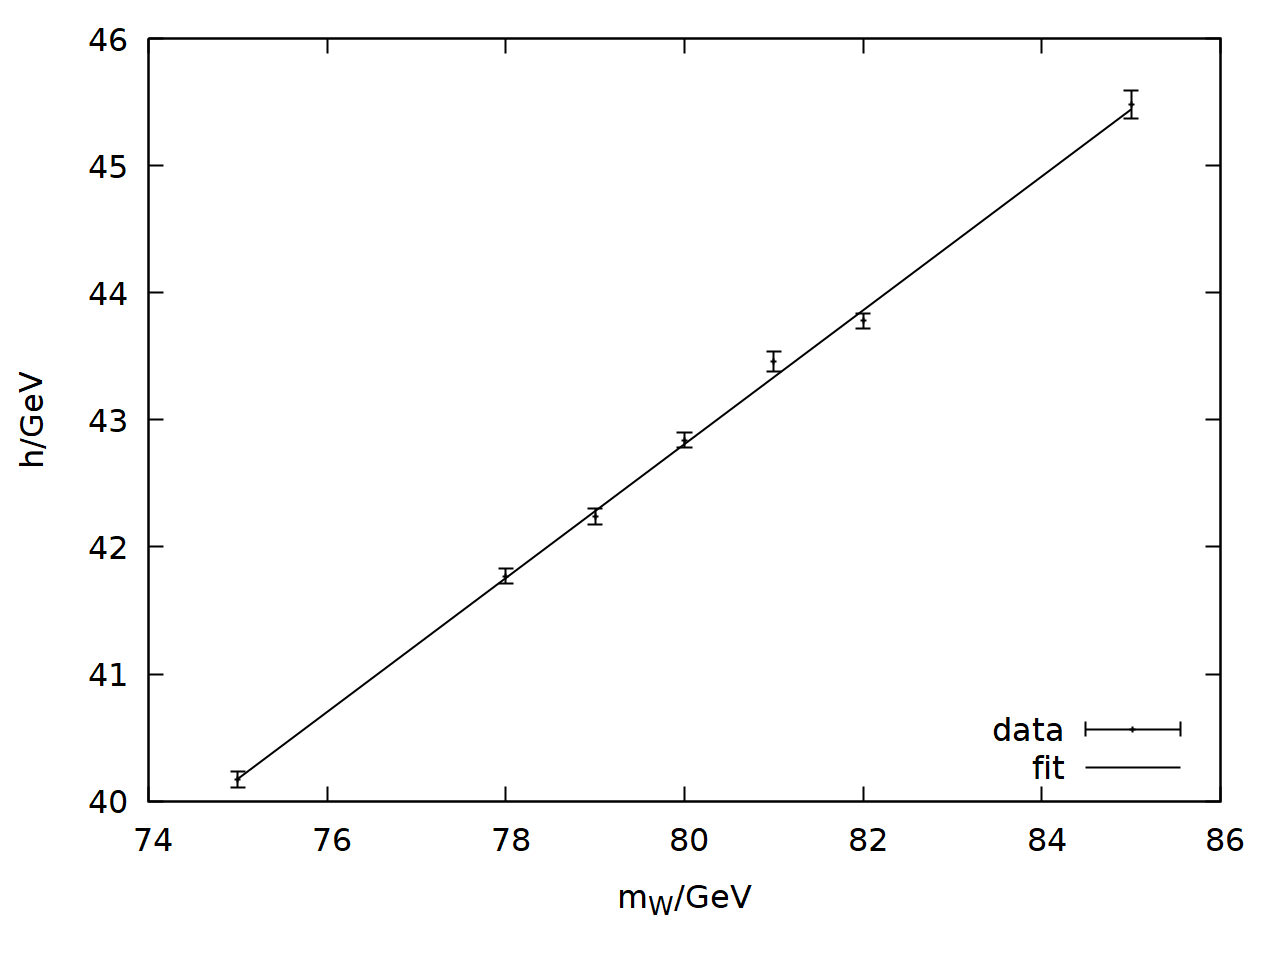
\includegraphics[width=0.7\textwidth]{data/33.png}
\caption{Linear Fit to the gauge curve}
\label{fig:task3_gauge}
\end{figure}

A linear fit $h = a\cdot m + b$ to this data (as seen in figure \ref{fig:task3_gauge}) yields $a = 0.53\pm 0.01, b = (0.7 \pm 0.8) \si{GeV})$.

The half maxima for the W boson data is $h = (42.77\pm 0.05)\,\si{GeV}$. Using the gauge curve fit this equals a W boson mass of $m\ind{W} = (79.93 \pm 2.05) \si{GeV} = (80 \pm 2)\,\si{GeV}$\footnote{The value with more decimal places will be useful when calculating the systematic errors.}.

The half maxima for the Z boson data is $h = (48.7 \pm 0.1)\,\si{GeV}$. This equals a Z boson mass of $m\ind{Z} = (91 \pm 2) \,\si{GeV}$. The PDG value for the Z boson mass is $m\ind{Z} = (91.1876 \pm 0.0021)\,\si{GeV}$. Therefore the real value lies within the error range of our result. This is used as a cross check for the gauge curve.

\subsubsection{Systematic error estimation}

We investigated the influence of the following parameters on the W boson mass: The QCD scale factor, the fit range width and the fit range position. These were the only parameters accessible to us. There are more systematic errors e.g. from the calibration as discussed in the lab instructions \cite{lab_instructions}.

\paragraph{Influence of the QCD scale factor}

Now we will investigate the influence of the QCD scale factor on the result. Therefore we repeated the whole calculations done in the last section for different QCD scale factors.

The result is plotted in figure \ref{fig:task3_qcd}.

\begin{figure}
\centering
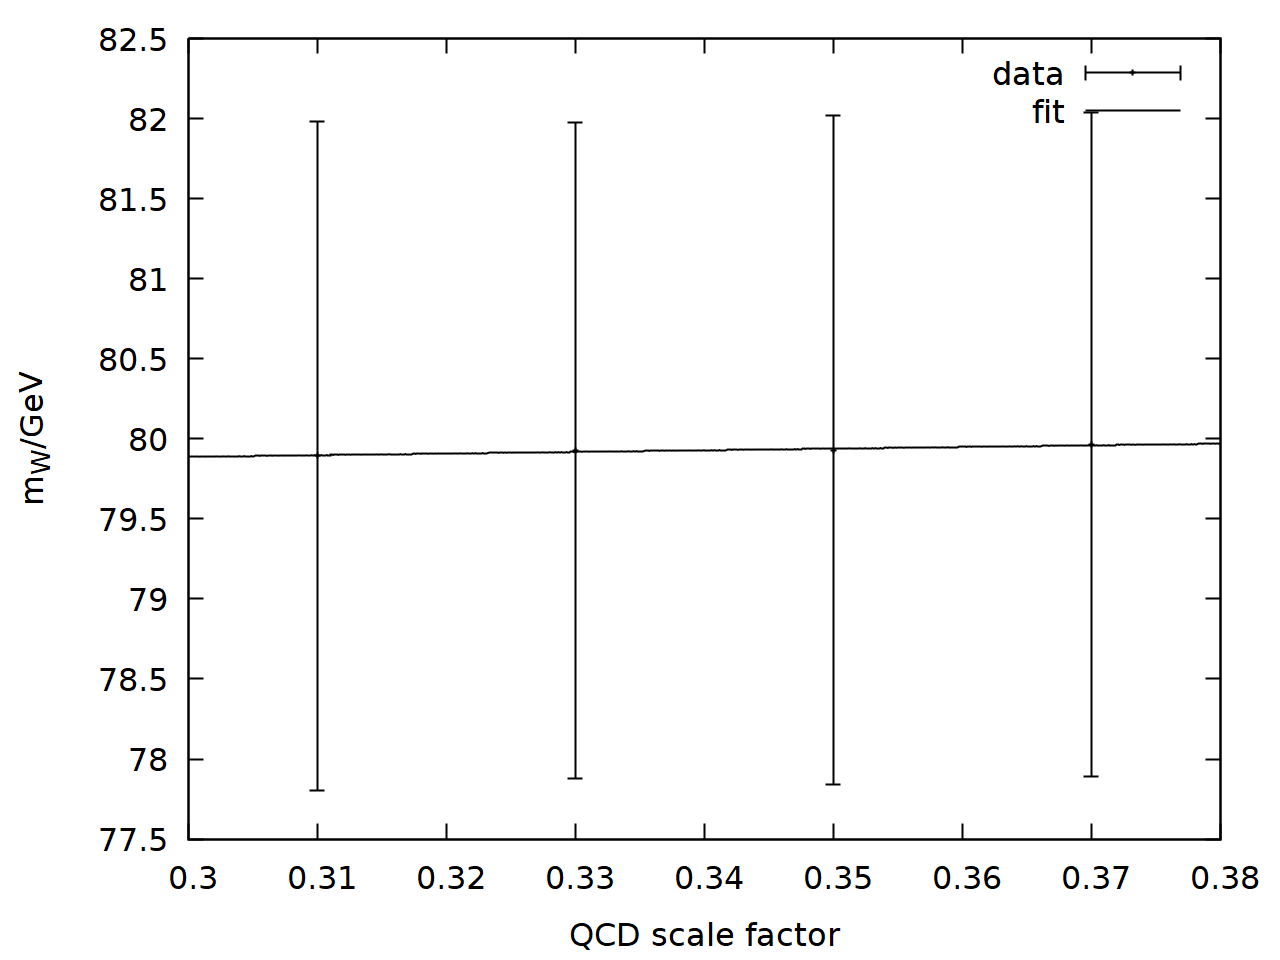
\includegraphics[width=0.7\textwidth]{data/qcdfactor.png}
\caption{Measured W boson mass over QCD scale factor}
\label{fig:task3_qcd}
\end{figure}

A linear fit $a\cdot x + b$ results in $a = (1 \pm 0.2)\,\si{GeV}$ and $b = (79.58 \pm 0.8) \, \si{GeV}$. Using this one can estimate the systematic error on the W boson mass $\delta m\ind{QCD} = a \cdot \Delta\alpha = 0.01 \si{GeV}$. 

\paragraph{Influence of a wider fit range}

Next we increased the fit range to $30 \si{GeV} - E_u$.  

The resulting masses are plotted in figure \ref{fig:task3_range}.

\begin{figure}
\centering
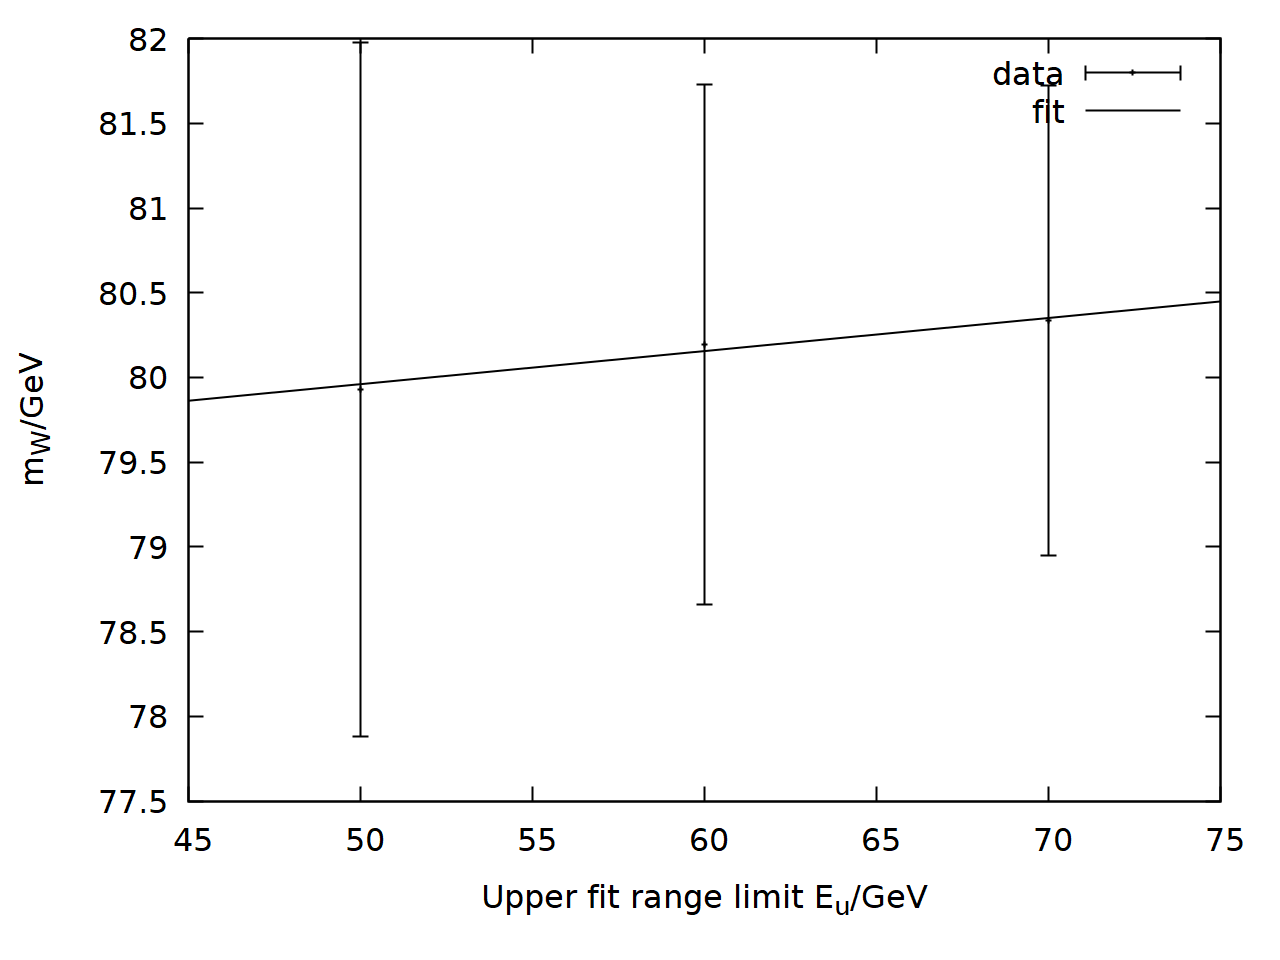
\includegraphics[width=0.7\textwidth]{data/range.png}
\caption{Measured W boson mass over fit range}
\label{fig:task3_range}
\end{figure}

A linear fit $a\cdot x + b$ results in $a = 0.020 \pm 0.003$ and $b = (79.0 \pm 0.2) \,\si{GeV}$. Using this one can estimate the systematic error on the W boson mass $\delta m\ind{Width} = a \cdot \Delta E_u = 0.1 \si{GeV}$. 

\paragraph{Influence of a shifted range}
To estimate the error due to the position of the range repeated the calculation with the range shifted to $35 - 55\,\si{GeV}$\footnote{We shifted it by $5\,\si{GeV}$ because we estimated the error of the range to $5\,\si{GeV}$}. We only shifted the interval ones because otherwise the half maximum ($\sim 40\,\si{GeV}$) would lie at the border of the interval.\\

The interval $35 - 55\,\si{GeV}$ resulted in a W boson mass $m_W = (80.10
\pm 3.73)\,\si{GeV} = (80 \pm 4)\,\si{GeV}$. The difference to our result for $30 - 50\,\si{GeV}$ is $\delta m\ind{Range} = 0.17\,\si{GeV}$.

\paragraph{Overall systematic error}
The overall systematic error is given by the sum of all systematic errors: $\delta m\ind{W} = \delta m\ind{QCD} + \delta m\ind{Width} + \delta m\ind{Range} = 0.18\, \si{GeV}$. 
 
\subsection{Result}

We determined the W boson mass to $m\ind{W} = m\ind{W}\,\pm\,\Delta m\ind{W}\,\pm\,\delta m\ind{W} = (79.93\,\pm\,2.05\,\pm\,0.18)\, \si{GeV} = \si{80 \pm 2 \pm 0.1}\, \si{GeV}$.

The statistical error $\Delta m\ind{W}$ is much bigger than the systematic error. The PDG value for the W boson mass is $m\ind{W} = (80.385 \pm 0.015)\,\si{GeV}$\cite{pdg}. Therefore the PDG value lies within the error bars of our result.
 
 